\chapter{System architecture}
\label{cha:architecture}

This section describes the system architecture of our solution.


% --------------------------------------------------------------------------- %
% Components
% --------------------------------------------------------------------------- %
\section{Components}
\label{sec:components}

Figure \ref{fig:class-diagram} show the structure of the components.

\begin{figure}
\begin{center}
	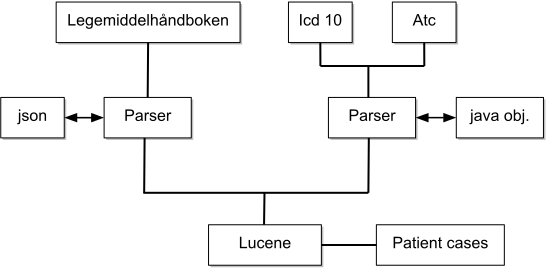
\includegraphics[width=\textwidth]{figures/class-diagram}
\end{center}
\caption{Class diagram}
\label{fig:class-diagram}
\end{figure}


% --------------------------------------------------------------------------- %
% External libraries
% --------------------------------------------------------------------------- %
\section{External libraries}
\label{sec:external-libraries}

\subsection*{Jsoup}
Jsoup is an open source java library for working with real-world HTML. It
provides a very convenient API for extracting and manipulating data. We use
Jsoup during the parsing of Legemiddelhåndboka.\\\\
\url{http://jsoup.org/}

\subsection*{The OWL API}
The OWL API is an open source java library used when working with owl
ontologies. We use this api when we’re retrieving information from the icd-10
owl ontology.\\\\
\url{http://owlapi.sourceforge.net/}

\subsection*{JSON.simple}
JSON simple is a java toolkit that are used to encode/decode JSON text. We use
this to when we want to save the chapters of Legemiddelhåndboka. We chose
JSON.simple because it provides a very simple and basic tool to convert java
objects to JSON text, which is just what we needed.\\\\
\url{https://code.google.com/p/json-simple/}

\subsection*{Lucene}
Apache Lucene is an open source text search engine library written in Java. We
use Lucene for all our indexing/searching operation in our solution.\\\\
\url{http://lucene.apache.org/core/}

% vim: set ts=2 sw=2 tw=80:
